% Reading Agent -- architecture overview (status: end of day 2, 2026-10-10)
% Self-contained; compile with pdflatex (e.g. on Overleaf).
\documentclass[11pt,a4paper]{article}
\usepackage[margin=2.2cm]{geometry}
\usepackage{amsmath,amssymb,bm}
\usepackage{booktabs}
\usepackage{xcolor}
\usepackage{hyperref}
\usepackage{enumitem}
\usepackage{float}
\usepackage{tikz}
\usetikzlibrary{arrows.meta,positioning,fit,backgrounds,calc,shapes.geometric}
\usepackage{pgfplots}
\pgfplotsset{compat=1.17}

\definecolor{tab}{HTML}{2E6FBF}
\definecolor{txt}{HTML}{C0662A}
\definecolor{rnn}{HTML}{3C8D5A}
\definecolor{head}{HTML}{8A4FB0}
\definecolor{frz}{HTML}{7A7A7A}

\tikzset{
  box/.style={draw, rounded corners=3pt, thick, align=center, minimum height=8mm, inner sep=4pt, font=\small},
  tabbox/.style={box, draw=tab, fill=tab!10},
  txtbox/.style={box, draw=txt, fill=txt!10},
  rnnbox/.style={box, draw=rnn, fill=rnn!12, minimum width=13mm},
  headbox/.style={box, draw=head, fill=head!10},
  frzbox/.style={box, draw=frz, fill=frz!12, dashed},
  arr/.style={-{Stealth[length=2.2mm]}, thick},
  darr/.style={-{Stealth[length=2.2mm]}, thick, dashed},
  lbl/.style={font=\scriptsize, align=center},
}

\newcommand{\htab}{h_{\mathrm{tab}}}

\title{\textbf{The Reading Agent}\\[2pt]
\large Tabular-conditioned active text reading for MulTaBench (Track 1)\\[2pt]
\normalsize Architecture and approach so far}
\author{NLP 097215 Final Project}
\date{Status: day 3 (2026-10-12)}

\begin{document}
\maketitle

\begin{abstract}
\noindent
A MulTaBench row has numeric and categorical columns plus one or more free-text fields.
We treat prediction as a sequential decision process.
The agent first reads the \emph{table}.
It then decides, one piece at a time, which pieces of text are worth reading, and it can stop at any step.
A table encoder initialises a stacked GRU.
Each text piece is a (column, sentence-chunk) item embedded once with frozen E5-small-v2.
An \emph{anytime predictor} outputs $\hat y$ after any number of reads.
An \emph{expected-gain head} estimates how much each unread item would lower the loss, and the agent reads greedily while that estimate exceeds a cost $\lambda$.
On women-clothing (fold 0), reading everything matches Joint Frozen.
At tight budgets, the learned policy beats a random reader by $+0.014$--$0.016$ AUROC.
\end{abstract}

%======================================================================
\section{Big picture}

\begin{figure}[h]
\centering
\resizebox{\linewidth}{!}{%
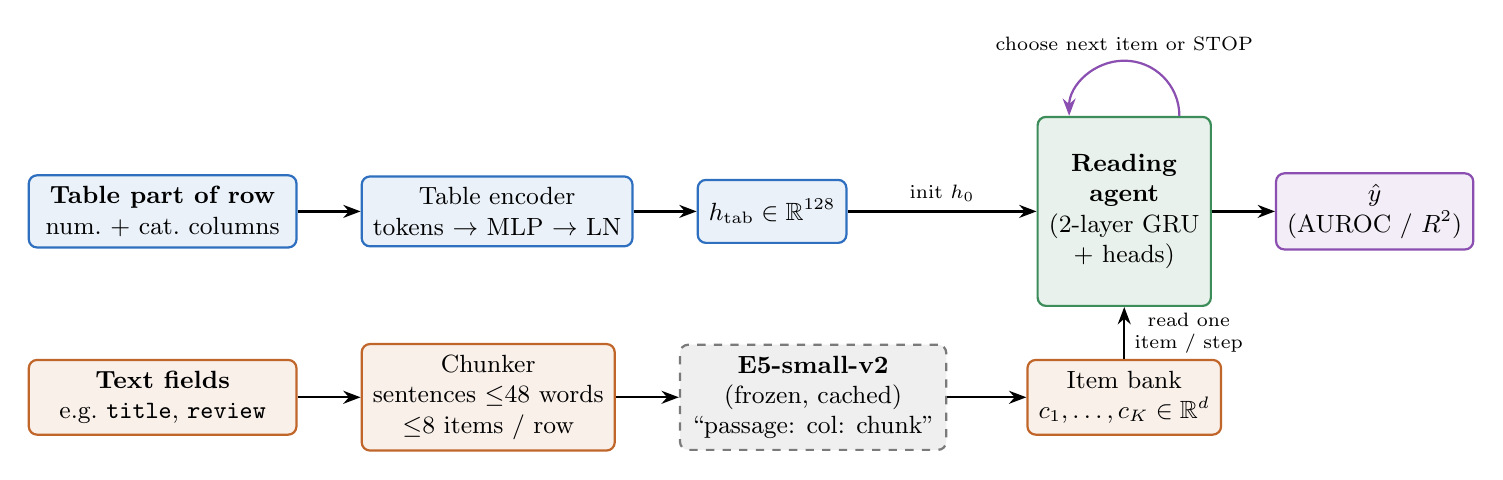
\begin{tikzpicture}[node distance=6mm and 8mm]
  % inputs
  \node[tabbox, minimum width=34mm] (row) {\textbf{Table part of row}\\num.\ + cat.\ columns};
  \node[txtbox, minimum width=34mm, below=14mm of row] (text) {\textbf{Text fields}\\e.g.\ \texttt{title}, \texttt{review}};

  % text pipeline
  \node[txtbox, right=of text] (chunk) {Chunker\\sentences $\le$48 words\\$\le$8 items / row};
  \node[frzbox, right=of chunk] (e5) {\textbf{E5-small-v2}\\(frozen, cached)\\``passage: col: chunk''};

  % table encoder
  \node[tabbox, right=of row] (tenc) {Table encoder\\tokens $\to$ MLP $\to$ LN};
  \node[tabbox, right=of tenc] (htab) {$\htab\in\mathbb{R}^{128}$};

  % agent
  \node[rnnbox, right=24mm of htab, minimum height=24mm, minimum width=22mm] (agent) {\textbf{Reading}\\\textbf{agent}\\(2-layer GRU\\+ heads)};
  \node[headbox, right=of agent] (yhat) {$\hat y$\\(AUROC / $R^2$)};
  \node[txtbox] (items) at (agent |- text) {Item bank\\$c_1,\dots,c_K\in\mathbb{R}^{d}$};

  \draw[arr] (row) -- (tenc);
  \draw[arr] (tenc) -- (htab);
  \draw[arr] (htab) -- node[lbl, above]{init $h_0$} (agent.west |- htab);
  \draw[arr] (text) -- (chunk);
  \draw[arr] (chunk) -- (e5);
  \draw[arr] (e5) -- (items);
  \draw[arr] (items.north) -- node[lbl, right]{read one\\item / step} (agent.south);
  \draw[arr] (agent) -- (yhat);
  \draw[arr, draw=head] ([xshift=7mm]agent.north) arc[start angle=0, end angle=180, radius=7mm]
    node[lbl, pos=0.5, above]{choose next item or STOP};
\end{tikzpicture}}
\caption{Overview. The table is always seen. Text is \emph{acquired} item by item, and the policy decides how much of it to read.}
\label{fig:overview}
\end{figure}

\noindent The design follows course concepts.
The encoder's output is the decoder's \emph{initial hidden state} (seq2seq, L9).
The model is a stacked GRU with inter-layer dropout (L8).
Reading is an MDP with a per-step cost, which acts like a length penalty (L11).
We tried imitation learning from an oracle with DAgger roll-ins (L11, T8) and then replaced it with value-of-information regression (\S\ref{sec:policy}).

%======================================================================
\section{Components}

\subsection{Items: what the agent can read}
Each text field is split into sentences.
Short sentences are merged greedily up to 48 words, and over-long sentences are cut into fixed 48-word windows.
A short field gives a single item.
Items are allocated round-robin across fields, up to $K\le 8$ per row.
Each item is verbalised as \texttt{"passage: <column>: <chunk>"}, the same format MulTaBench uses.
It is embedded \emph{once} with frozen E5-small-v2 ($384$-d) and cached to disk.
Inside the model, item $i$ becomes
\[
  c_i=\mathrm{LN}\big(W_{\mathrm{item}}\,e_i \;+\; W_{\mathrm{name}}\,\mathrm{E5}(\text{field name}) \;+\; p_{\mathrm{pos}(i)}\big)\in\mathbb{R}^{128}.
\]

\subsection{Table encoder $\to$ initial state}
\begin{figure}[h]
\centering
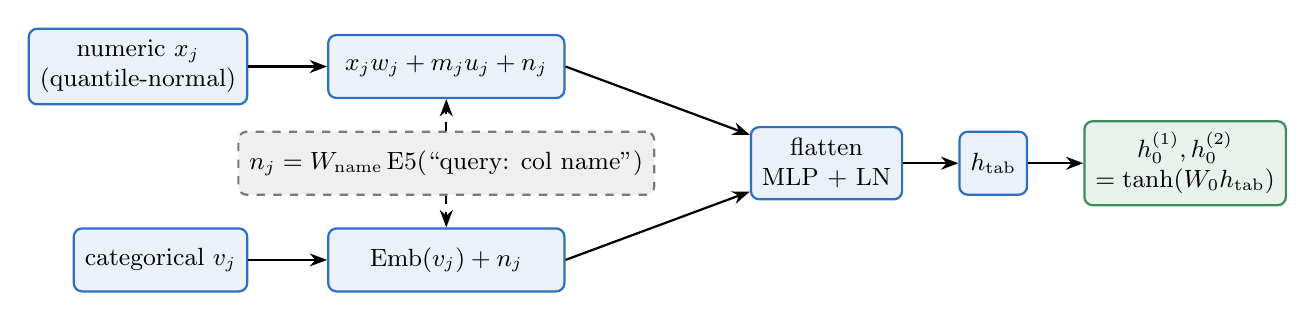
\begin{tikzpicture}[node distance=5mm and 7mm]
  \node[tabbox, minimum width=30mm] (tn) {$x_j w_j + m_j u_j + n_j$};
  \node[frzbox, below=4mm of tn] (cn) {$n_j=W_{\mathrm{name}}\,$E5(``query: col name'')};
  \node[tabbox, below=4mm of cn, minimum width=30mm] (tc) {$\mathrm{Emb}(v_j) + n_j$};
  \node[tabbox, left=10mm of tn] (num) {numeric $x_j$\\(quantile-normal)};
  \node[tabbox, left=10mm of tc] (cat) {categorical $v_j$};
  \node[tabbox, right=12mm of cn] (mlp) {flatten\\MLP + LN};
  \node[tabbox, right=of mlp] (ht) {$\htab$};
  \node[rnnbox, right=of ht] (h0) {$h_0^{(1)},h_0^{(2)}$\\$=\tanh(W_0\htab)$};
  \draw[arr] (num) -- (tn);
  \draw[arr] (cat) -- (tc);
  \draw[darr] (cn) -- (tn);
  \draw[darr] (cn) -- (tc);
  \draw[arr] (tn.east) -- (mlp);
  \draw[arr] (tc.east) -- (mlp);
  \draw[arr] (mlp) -- (ht);
  \draw[arr] (ht) -- (h0);
\end{tikzpicture}
\caption{Table encoder. $m_j$ is the missing indicator, and $n_j$ is the projected column-name embedding.
With no table columns, a learned null vector is used.}
\end{figure}

\subsection{The read loop (unrolled)}
\begin{figure}[h]
\centering
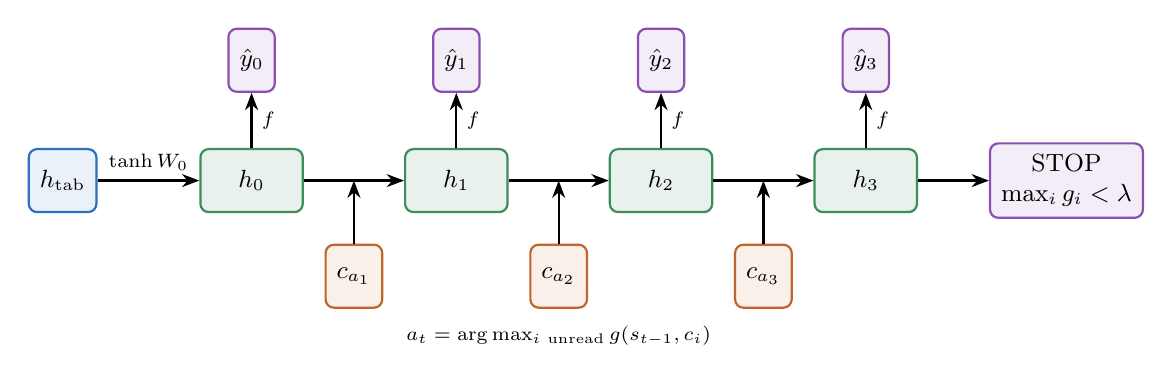
\begin{tikzpicture}[node distance=4mm and 9mm]
  \node[tabbox] (ht) {$\htab$};
  \foreach \t/\x in {0/0,1/1,2/2,3/3} {
    \node[rnnbox] (g\t) at ($(ht)+(2.4+2.6*\x,0)$) {$h_{\t}$};
    \node[headbox, above=7mm of g\t] (p\t) {$\hat y_{\t}$};
    \draw[arr] (g\t) -- node[lbl, right]{$f$} (p\t);
  }
  \draw[arr] (ht) -- node[lbl, above]{$\tanh W_0$} (g0);
  \coordinate (m1) at ($(g0)!0.5!(g1)$);
  \coordinate (m2) at ($(g1)!0.5!(g2)$);
  \coordinate (m3) at ($(g2)!0.5!(g3)$);
  \node[txtbox, below=8mm of m1] (c1) {$c_{a_1}$};
  \node[txtbox, below=8mm of m2] (c2) {$c_{a_2}$};
  \node[txtbox, below=8mm of m3] (c3) {$c_{a_3}$};
  \draw[arr] (g0) -- (g1); \draw[arr] (g1) -- (g2); \draw[arr] (g2) -- (g3);
  \draw[arr] (c1) -- (m1);
  \draw[arr] (c2) -- (m2);
  \draw[arr] (c3) -- (m3);
  \node[headbox, right=9mm of g3] (stop) {STOP\\$\max_i g_i<\lambda$};
  \draw[arr] (g3) -- (stop);
  \node[lbl, below=1mm of c2] {$a_t=\arg\max_{i\ \text{unread}} g(s_{t-1},c_i)$};
\end{tikzpicture}
\caption{Unrolled reading. Each step feeds one chosen item into the 2-layer GRU.
The predictor $f$ can be queried after every step, so the model is an \emph{anytime} predictor.}
\end{figure}

The state summary after $t$ reads is
\[
  s_t=\big[\,h^{(2)}_t\;;\;\tfrac{1}{t}\textstyle\sum_{\tau\le t}c_{a_\tau}\;;\;\htab\,\big]\in\mathbb{R}^{384},
\]
and all heads read from it:
\begin{itemize}[nosep]
  \item \textbf{Predictor} $f(s_t)$: an MLP ($384\to256\to n_{\text{out}}$, GELU, dropout).
  \item \textbf{Expected-gain head} $g(s_t,k_i)=\mathrm{MLP}([s_t;k_i])$, the predicted reduction in loss from reading item $i$ next.
        The key $k_i$ is either the item itself (\emph{content} keys) or only its field and position (\emph{meta} keys, a true feature-acquisition setting in which content is unseen before reading).
\end{itemize}

%======================================================================
\section{Training}

\begin{figure}[h]
\centering
\resizebox{\linewidth}{!}{%
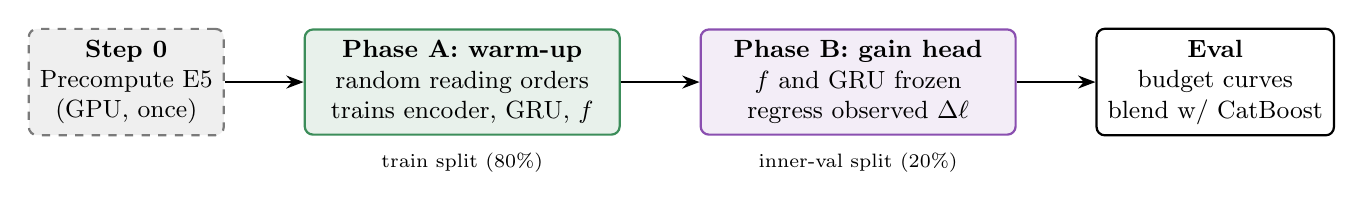
\begin{tikzpicture}[node distance=6mm and 10mm]
  \node[frzbox] (pre) {\textbf{Step 0}\\Precompute E5\\(GPU, once)};
  \node[rnnbox, right=of pre, minimum width=40mm] (A) {\textbf{Phase A: warm-up}\\random reading orders\\trains encoder, GRU, $f$};
  \node[headbox, right=of A, minimum width=40mm] (B) {\textbf{Phase B: gain head}\\$f$ and GRU frozen\\regress observed $\Delta\ell$};
  \node[box, right=of B] (ev) {\textbf{Eval}\\budget curves\\blend w/ CatBoost};
  \draw[arr] (pre) -- (A); \draw[arr] (A) -- (B); \draw[arr] (B) -- (ev);
  \node[lbl, below=1mm of A] {train split (80\%)};
  \node[lbl, below=1mm of B] {inner-val split (20\%)};
\end{tikzpicture}}
\end{figure}

\paragraph{Phase A (warm-up).}
For each batch, sample a random reading order and unroll over all items.
The loss mixes every prefix with the full read:
\[
  \mathcal{L}_A=\tfrac12\cdot\frac{1}{K+1}\sum_{t=0}^{K}\ell\big(f(s_t),y\big)\;+\;\tfrac12\,\ell\big(f(s_K),y\big).
\]
The loss $\ell$ is cross-entropy for classification and MSE for regression.
We train with AdamW (lr $10^{-3}$), clip gradients at norm 1, and early-stop on the val loss of the full read.
Random orders make $f$ reliable after \emph{any} subset of reads, which the policy needs.

\paragraph{Phase B (expected-gain policy).}\label{sec:policy}
With $f$ frozen, roll in $\varepsilon$-greedily ($\varepsilon=0.3$) using the current $g$.
At every visited state, compute the observed one-step gain of every unread item $i$:
\[
  \Delta_i(s_t)=\ell\big(f(s_t),y\big)-\ell\big(f(s_t\oplus c_i),y\big),
  \qquad
  \mathcal{L}_B=\sum_{t,\,i\ \text{unread}}\big(g(s_t,k_i)-\Delta_i(s_t)\big)^2 .
\]
The label is needed only to build the regression \emph{targets}.
At test time $g$ estimates $\mathbb{E}[\Delta\mid s_t,k_i]$ without $y$, which is a label-free value-of-information estimate.
The head is fit on the 20\% inner-validation split because $f$'s in-sample losses are biased low.
Rolling in with the agent's own policy (DAgger-style) keeps the training states on the test-time distribution.
\textbf{Inference:} read $\arg\max_i g$ while $\max_i g\ge\lambda$.
Sweeping $\lambda$ traces an accuracy-versus-budget curve.

\paragraph{Why not imitation? (negative result).}
Our first policy was a pointer network with a STOP key, trained to imitate a greedy \emph{label} oracle.
The oracle picks the item that most lowers the loss for the \emph{true} $y$.
Its choices depend on $y$, so a policy that cannot see $y$ cannot imitate them.
In practice the imitation policy did no better than random at every $\lambda$.
The oracle's own AUROC of $0.966$ with $1.5$ reads reflects cherry-picking by label, so it is not an achievable upper bound.
Regressing the \emph{expected} gain removes this problem.

%======================================================================
\section{Evaluation setup and baselines}
\begin{itemize}[nosep]
  \item MulTaBench text datasets (20), with the official repeated 3-fold $\times2$ splits (seed 42) vendored in the code.
        Metrics are AUROC (macro OvR for multiclass) and $R^2$.
  \item \textbf{Agent modes:} table only ($t=0$), read-all, gain@$\lambda$, random at a matched per-row budget, and the label oracle (diagnostic only).
  \item \textbf{Baselines:} CatBoost Joint-Frozen (num + cat + PCA-30 of whole-field E5 per text column), CatBoost tab-only, table-conditioned soft attention over all items, OOF stacking, and a val-tuned convex blend of CatBoost and the agent.
  \item \textbf{Bar to beat:} the method is target-aware, so the relevant bar is \emph{Joint TAR}.
        We also report against Joint Frozen (official leaderboard CSVs, Wilcoxon over dataset $\times$ fold).
\end{itemize}

%======================================================================
\section{Results so far (women-clothing, fold 0)}

\begin{table}[H]
\centering
\begin{tabular}{lc}
\toprule
Model & AUROC \\
\midrule
CatBoost tab-only & 0.7825 \\
Agent, table only (no reads) & 0.7826 \\
Soft attention over all items & 0.8976 \\
Agent, read-all & 0.8990 \\
CatBoost Joint-Frozen (ours / leaderboard) & 0.9024 / 0.9028 \\
OOF stacking & 0.9032 \\
\textbf{Val-tuned blend CatBoost + agent} & \textbf{0.9046} \\
\midrule
CatBoost Joint-TAR (leaderboard) & $\approx$0.909 \\
\bottomrule
\end{tabular}
\caption{Accuracy. Our CatBoost Frozen reproduces the leaderboard, which validates the pipeline.}
\end{table}

\begin{figure}[H]
\centering
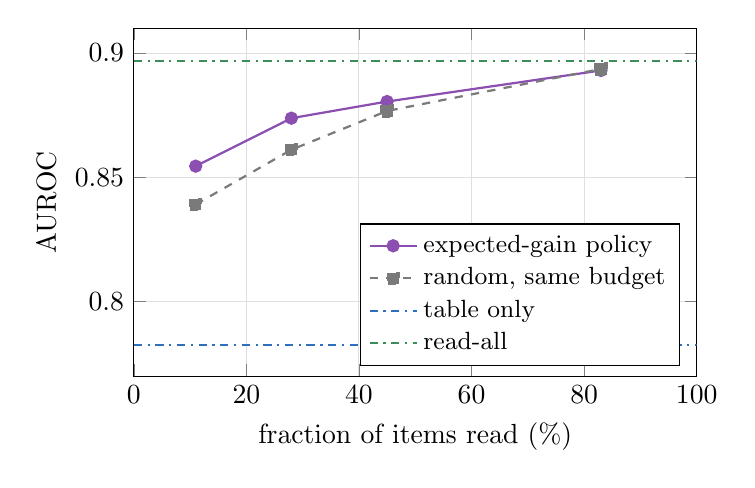
\begin{tikzpicture}
\begin{axis}[
  width=0.72\linewidth, height=6cm,
  xlabel={fraction of items read (\%)}, ylabel={AUROC},
  xmin=0, xmax=100, ymin=0.77, ymax=0.91,
  legend pos=south east, legend cell align=left, legend style={font=\small},
  grid=major, grid style={gray!25},
]
\addplot[thick, color=head, mark=*] coordinates {(11,0.8545) (28,0.8738) (45,0.8805) (83,0.8930)};
\addlegendentry{expected-gain policy}
\addplot[thick, color=frz, mark=square*, dashed] coordinates {(11,0.8391) (28,0.8611) (45,0.8767) (83,0.8936)};
\addlegendentry{random, same budget}
\addplot[thick, color=tab, dash dot, domain=0:100, samples=2] {0.7826};
\addlegendentry{table only}
\addplot[thick, color=rnn, dash dot, domain=0:100, samples=2] {0.8969};
\addlegendentry{read-all}
\end{axis}
\end{tikzpicture}
\caption{Accuracy versus reading budget (experiment \#3, content keys).
The learned policy's advantage grows as the budget shrinks ($+0.016$ at 11\% of items read).
Near full budget the advantage is unstable across initialisations.
Meta keys stay close to random.}
\end{figure}

%======================================================================
\section{Iteration log (day 3, 2026-10-12)}

\paragraph{Fixes.}
A static audit found a bug in the gain-head loss.
The loss was normalised by a count that kept growing across the batches of an epoch, which silently decayed the learning rate within each epoch.
It now uses a per-batch mean.
Other fixes:
\begin{itemize}[nosep]
  \item Multiclass AUROC is computed over the classes present in the test set; before, a missing class gave NaN.
  \item CatBoost class names are fixed in advance.
  \item Each run has an id, and runs without a completion marker are ignored when results are aggregated.
\end{itemize}

\paragraph{Budget-targeted curves.}
A $\lambda$ grid means different budgets on different datasets.
We therefore bisect $\lambda$ on the validation split to hit target read fractions of $10/25/50/75\%$.
This needs only $g$, not labels.

\begin{table}[H]
\centering
\small
\begin{tabular}{llcccc}
\toprule
Dataset (fold 0) & Variant & table only & read-all & CB Frozen & blend \\
\midrule
fake-job & default & 0.695 & 0.867 & 0.915 & 0.919 \\
fake-job & + field meta & \textbf{0.761} & 0.858 & 0.915 & 0.920 \\
fake-job & + plateau lr & 0.702 & 0.854 & 0.915 & 0.915 \\
fake-job & whole-field items & 0.687 & 0.863 & -- & -- \\
women-clothing & default & 0.783 & 0.899 & 0.902 & 0.905 \\
women-clothing & + plateau lr & 0.783 & 0.897 & 0.902 & 0.904 \\
\bottomrule
\end{tabular}
\caption{Ablations. ``Field meta'' gives the table encoder a presence flag and the log length of each text field.}
\end{table}

\begin{table}[H]
\centering
\small
\begin{tabular}{llcccc}
\toprule
Dataset & Variant & 10\% & 25\% & 50\% & 75\% \\
\midrule
fake-job & default & +0.024 & +0.015 & +0.017 & +0.004 \\
fake-job & + field meta & $-$0.005 & $-$0.003 & $-$0.003 & $-$0.001 \\
women-clothing & default & +0.013 & +0.012 & +0.006 & +0.001 \\
\bottomrule
\end{tabular}
\caption{AUROC advantage of the gain policy (content keys) over random reading at the same per-row budget.}
\end{table}

\paragraph{Findings.}
\begin{enumerate}[nosep]
  \item \textbf{The gain policy generalises} from women-clothing to fake-job, and its advantage is largest at tight budgets.
  \item \textbf{Part of that advantage is metadata.}
        When the table encoder already knows which fields exist and how long they are, the policy's edge over random disappears on fake-job.
        A large share of the value of information there is ``read the fields that exist / are long''.
        This should be stated honestly in the paper.
  \item \textbf{The read-all gap to CatBoost on fake-job ($\approx0.05$) is in the learner, not the chunking.}
        Whole-field items, which are exactly the strings CatBoost embeds, give the same read-all AUROC.
        The warm-up validation loss is very noisy on this imbalanced dataset.
        A plateau LR schedule did not help.
  \item \textbf{Fake-job varies by $\pm0.01$ from run to run}, so conclusions need the multi-dataset, multi-fold sweep.
\end{enumerate}

%======================================================================
\section{Status and next steps}
\begin{enumerate}[nosep]
  \item Embedding cache: 15 of 20 datasets are done (wine was added on day 3).
        Five remain: kickstarter, us-accidents, mercari, jigsaw and spotify.
  \item Fold-0 sweep over the 15 cached datasets (recipe locked: no field meta, no schedule, budget curves).
        The first attempt was killed by the system's low-memory reaper.
  \item Finish the gain-head ablation (val vs.\ train+val, 15 vs.\ 40 epochs) and lock the recipe.
  \item Sweep 20 datasets $\times$ folds 0--2, then compare to the leaderboard with Wilcoxon tests.
  \item Paper framing: \emph{tabular-conditioned active text reading}.
        Headline results are the budget curves, the blend versus Frozen, and an honest comparison with TAR.
\end{enumerate}

\end{document}
